\documentclass[aspectratio=169]{beamer}

% Shared Beamer settings for Elements of AIML lectures (UPES).
% Keep this file free of \documentclass to allow reuse via \input.

% Allow lecture sources to use shared theme/assets without copying them into each lecture folder.
% NOTE: These paths are relative to `Unit-xx/Lecture-yy/latex/` (and `Lab/Experiment-xx/latex/`).
\makeatletter
\def\input@path{{../../../_shared/}{../../../_shared/UPES-Beamer-Theme/}}
\makeatother

\usetheme{UPES}
\setbeamertemplate{navigation symbols}{}

\usepackage{amsmath}
\usepackage{amssymb}
\usepackage{booktabs}
\usepackage{graphicx}
\usepackage{hyperref}
\usepackage{xcolor}
\usepackage{listings}

% Code listings (general-purpose).
\lstset{
  basicstyle=\ttfamily\small,
  keywordstyle=\color{blue},
  commentstyle=\color{gray},
  stringstyle=\color{teal},
  showstringspaces=false,
  columns=fullflexible,
  breaklines=true
}

\usepackage{tikz}
\usetikzlibrary{arrows.meta,positioning,shapes.geometric,calc}

% Per-slide source line (references shown on the slide itself).
\newcommand{\slidesources}[1]{%
  \vfill
  {\tiny\color{gray}\raggedright\sloppy\parbox{\linewidth}{Sources: #1}\par}%
}

% Unit-wise source strings for this subject (used by slides/notes).
% Path is relative to the lecture `latex/` folder (the compilation CWD).
% Source strings for Elements of AIML (used by slides + notes).

\newcommand{\AIMLRepoURL}{https://github.com/tali7c/Elements-of-AIML}

\newcommand{\AIMLLabSources}{%
Provost and Fawcett, \textit{Data Science for Business}.;%
McKinney, \textit{Python for Data Analysis}.;%
WEKA Documentation (Waikato Environment for Knowledge Analysis), accessed 2026-02-28.;%
Matplotlib and Seaborn documentation, accessed 2026-02-28.%
}

\newcommand{\AIMLUnitISources}{%
Rich and Knight, \textit{Artificial Intelligence}, McGraw Hill, 2017.;%
Russell and Norvig, \textit{Artificial Intelligence: A Modern Approach} (4e), Ch. 1--2 (Introduction, Intelligent Agents).;%
Poole and Mackworth, \textit{Artificial Intelligence: Foundations of Computational Agents} (2e), selected sections.%
}

\newcommand{\AIMLUnitIISources}{%
Russell and Norvig, \textit{Artificial Intelligence: A Modern Approach} (4e), Ch. 7--9 (Logical Agents, First-Order Logic, Inference).;%
Huth and Ryan, \textit{Logic in Computer Science} (2e), selected sections on propositional and first-order logic.;%
Genesereth and Nilsson, \textit{Logical Foundations of Artificial Intelligence}, selected chapters.%
}

\newcommand{\AIMLUnitIIISources}{%
Mueller and Massaron, \textit{Machine Learning for Dummies}, For Dummies, 2016.;%
Mitchell, \textit{Machine Learning}, selected chapters on learning basics and evaluation.;%
Scikit-learn documentation, accessed 2026-02-28.%
}

\newcommand{\AIMLUnitIVSources}{%
Mueller and Massaron, \textit{Machine Learning for Dummies}, For Dummies, 2016.;%
James, Witten, Hastie, and Tibshirani, \textit{An Introduction to Statistical Learning} (2e), selected chapters.;%
Scikit-learn documentation, accessed 2026-02-28.%
}

\newcommand{\AIMLUnitVSources}{%
NIST, \textit{AI Risk Management Framework (AI RMF 1.0)}, 2023.;%
Barocas, Hardt, and Narayanan, \textit{Fairness and Machine Learning} (online book), selected sections.;%
Knaflic, \textit{Storytelling with Data}, selected chapters on communicating results.%
}



\title[Elements of AIML]{Elements of AIML}
\subtitle{Unit 02 -- Lecture 01: Propositional Logic Foundations (Entailment)}
\author{Tofik Ali}
\institute{School of Computer Science, UPES Dehradun}
\date{\today}

\graphicspath{{../images/}{../../../_shared/}{../../../_shared/UPES-Beamer-Theme/}}

\begin{document}

\UPESCoverFrame
\setcounter{framenumber}{0}

\begin{frame}
  \titlepage
  \vspace{0.3em}
  \begin{center}
    \footnotesize Topic focus: \textbf{Logic for AI} (syntax, semantics, and basic inference)\\[0.25em]
    \footnotesize Repository: \texttt{\AIMLRepoURL}
  \end{center}
  \slidesources{\AIMLUnitIISources}
\end{frame}

\begin{frame}{Quick Links}
  \centering
  \hyperlink{sec:overview}{\beamerbutton{Overview}}\hspace{0.6em}
  \hyperlink{sec:pl}{\beamerbutton{Propositional}}\hspace{0.6em}
  \hyperlink{sec:limits}{\beamerbutton{Limits}}\hspace{0.6em}
  \hyperlink{sec:practice}{\beamerbutton{Practice}}\hspace{0.6em}
  \hyperlink{sec:summary}{\beamerbutton{Summary}}
\end{frame}

\begin{frame}{Agenda}
  \tableofcontents
\end{frame}

\section{Overview}
\label{sec:overview}

\begin{frame}{Learning Outcomes}
  By the end of this lecture, you should be able to:
  \begin{itemize}[<+->]
    \item Define \textbf{propositions} and build compound statements using logical connectives.
    \item Construct and use \textbf{truth tables} to test validity, satisfiability, and equivalence (basic cases).
    \item Explain \textbf{entailment} ($KB \models \alpha$) and how to check it using models (small KBs).
    \item Convert simple formulas to \textbf{CNF} (preview of automated inference).
    \item Explain (at a high level) why propositional logic is insufficient for many AI knowledge bases.
  \end{itemize}
\end{frame}

\begin{frame}{Abbreviations \& Symbols}
  \begin{itemize}[<+->]
    \item $KB$: knowledge base,\; $\alpha$: query/goal sentence
    \item $\models$: semantic entailment,\; $\vdash$: derivation/provability
    \item $\lnot,\land,\lor,\rightarrow,\leftrightarrow$: NOT, AND, OR, IMPLIES, IFF
    \item PL: propositional logic,\; CNF: conjunctive normal form
  \end{itemize}
\end{frame}

\begin{frame}{Why Logic in AI?}
  \begin{itemize}[<+->]
    \item AI systems often need \textbf{explicit knowledge}: facts + rules (a \textbf{knowledge base}).
    \item Logic provides a precise way to ask: \textit{``Does my knowledge base imply this query?''}
    \item Separates:
    \begin{itemize}
      \item \textbf{Representation} (what we say),
      \item \textbf{Reasoning} (how we derive consequences).
    \end{itemize}
  \end{itemize}
  \vspace{0.4em}
  \centering
  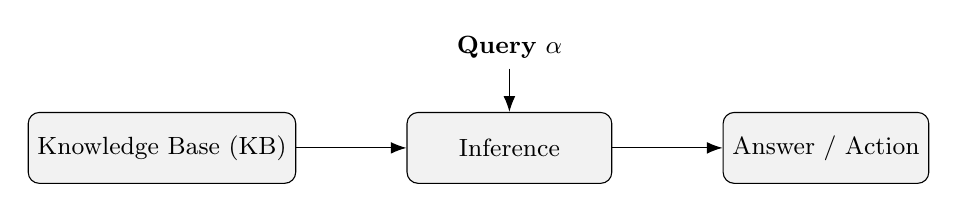
\begin{tikzpicture}[node distance=1.4cm, every node/.style={font=\small}]
    \node (kb) [draw, rounded corners, fill=gray!10, minimum width=2.6cm, minimum height=0.9cm] {Knowledge Base (KB)};
    \node (inf) [draw, rounded corners, right=of kb, fill=gray!10, minimum width=2.6cm, minimum height=0.9cm] {Inference};
    \node (ans) [draw, rounded corners, right=of inf, fill=gray!10, minimum width=2.6cm, minimum height=0.9cm] {Answer / Action};
    \draw[-{Latex[length=2mm]}] (kb) -- (inf);
    \draw[-{Latex[length=2mm]}] (inf) -- (ans);
    \node (q) [above=0.55cm of inf] {\textbf{Query} $\alpha$};
    \draw[-{Latex[length=2mm]}] (q) -- (inf);
  \end{tikzpicture}
\end{frame}

\begin{frame}{Two Levels: Syntax vs Semantics}
  \begin{itemize}[<+->]
    \item \textbf{Syntax}: the legal \emph{forms} of sentences (symbols + grammar).
    \item \textbf{Semantics}: what sentences \emph{mean} (truth under an interpretation/model).
    \item In AI we care about \textbf{entailment}:
    \[
      KB \models \alpha \quad \text{(in every model where $KB$ is true, $\alpha$ is true).}
    \]
  \end{itemize}
\end{frame}

\section{Propositional Logic}
\label{sec:pl}

\begin{frame}{Propositional Logic: What It Can Express}
  \begin{itemize}[<+->]
    \item A \textbf{proposition} is a declarative statement that is either \textbf{True} or \textbf{False}.
    \item Examples:
    \begin{itemize}
      \item $p$: ``It is raining.''
      \item $q$: ``The ground is wet.''
    \end{itemize}
    \item We build compound sentences using \textbf{connectives}:
    \[
      \lnot p,\; p \land q,\; p \lor q,\; p \rightarrow q,\; p \leftrightarrow q
    \]
  \end{itemize}
\end{frame}

\begin{frame}{Truth Tables (Core Tool)}
  \begin{itemize}[<+->]
    \item Truth tables enumerate all assignments of truth values to variables.
    \item They let us check:
    \begin{itemize}
      \item \textbf{Tautology}: always true
      \item \textbf{Contradiction}: always false
      \item \textbf{Satisfiable}: true in at least one assignment (has a model)
    \end{itemize}
  \end{itemize}
\end{frame}

\begin{frame}{Implication ($p \rightarrow q$) Confusion Fix}
  $p \rightarrow q$ is \textbf{false only when} $p$ is true and $q$ is false.

  \vspace{0.6em}
  \centering
  \begin{tabular}{cc|c}
    \toprule
    $p$ & $q$ & $p \rightarrow q$ \\
    \midrule
    T & T & T \\
    T & F & F \\
    F & T & T \\
    F & F & T \\
    \bottomrule
  \end{tabular}

  \vspace{0.6em}
  Key equivalence:
  \[
    (p \rightarrow q) \equiv (\lnot p \lor q)
  \]
\end{frame}

\begin{frame}{Worked Truth Table (Example)}
  Example formula: $(p \land q) \lor \lnot p$

  \vspace{0.6em}
  \centering
  \begin{tabular}{cc|c|c|c}
    \toprule
    $p$ & $q$ & $p \land q$ & $\lnot p$ & $(p \land q) \lor \lnot p$ \\
    \midrule
    T & T & T & F & T \\
    T & F & F & F & F \\
    F & T & F & T & T \\
    F & F & F & T & T \\
    \bottomrule
  \end{tabular}
\end{frame}

\begin{frame}{Equivalence Laws (Selected)}
  \begin{itemize}[<+->]
    \item De Morgan:
    \[
      \lnot(p \land q) \equiv (\lnot p \lor \lnot q), \quad
      \lnot(p \lor q) \equiv (\lnot p \land \lnot q)
    \]
    \item Distributive:
    \[
      p \land (q \lor r) \equiv (p \land q) \lor (p \land r)
    \]
    \item Double negation: $\lnot(\lnot p) \equiv p$
  \end{itemize}
\end{frame}

\begin{frame}{Normal Forms: CNF vs DNF}
  \begin{itemize}[<+->]
    \item \textbf{CNF} (Conjunctive Normal Form): AND of OR-clauses
    \[
      (a \lor b \lor \lnot c) \land (\lnot a \lor d)
    \]
    \item \textbf{DNF} (Disjunctive Normal Form): OR of AND-terms
    \[
      (a \land b) \lor (\lnot a \land c)
    \]
    \item Many inference procedures (e.g., \textbf{resolution}) expect CNF.
  \end{itemize}
\end{frame}

\begin{frame}{CNF Conversion (Mini Example)}
  Convert: $(p \rightarrow q) \land p$
  \begin{itemize}[<+->]
    \item Eliminate implication: $(\lnot p \lor q) \land p$
    \item Already in CNF:
    \[
      (\lnot p \lor q) \land (p)
    \]
  \end{itemize}
  This is the standard form used for many automated checks.
\end{frame}

\begin{frame}{Inference: Entailment vs Derivation}
  \begin{itemize}[<+->]
    \item \textbf{Semantic entailment}: $KB \models \alpha$ (meaning-based, via models).
    \item \textbf{Syntactic derivation}: $KB \vdash \alpha$ (proof-based, via rules).
    \item Example (Modus Ponens):
    \[
      (p \rightarrow q),\; p \;\;\vdash\;\; q
    \]
  \end{itemize}
\end{frame}

\begin{frame}{Checkpoint \#1 (30 seconds)}
  \textbf{Given:} $KB = \{(p \rightarrow q), (q \rightarrow r), p\}$

  \vspace{0.6em}
  \textbf{Question:} Does $KB \models r$? Briefly justify (1--2 lines).
\end{frame}

\section{Limits of propositional logic (preview)}
\label{sec:limits}

\begin{frame}{Why Propositional Logic Becomes Insufficient}
  Propositional logic is great for \textbf{small} worlds, but it struggles when we need:
  \begin{itemize}[<+->]
    \item \textbf{Many objects}: one symbol per object-fact becomes too verbose
    \item \textbf{Relations}: ``$x$ is parent of $y$'' cannot be expressed naturally
    \item \textbf{Quantification}: ``all'' / ``some'' statements cannot be expressed compactly
  \end{itemize}
  \vspace{0.3em}
  Next lecture: \textbf{predicate (first-order) logic} solves these with objects, predicates, and quantifiers.
\end{frame}

\begin{frame}{Preview: What Predicate Logic Adds (One Slide)}
  \begin{itemize}[<+->]
    \item Predicates: $Student(x)$, $Enrolled(x,y)$
    \item Quantifiers: $\forall$ (for all), $\exists$ (there exists)
    \item Example rule (compact):
    \[
      \forall x\; (Human(x) \rightarrow Mortal(x))
    \]
  \end{itemize}
  We will do full syntax, semantics, and translation in \textbf{Lecture 02}.
\end{frame}

\section{Practice}
\label{sec:practice}

\begin{frame}[fragile]{Mini Demo (Propositional Logic by Brute Force)}
  We can check entailment by enumerating truth assignments (small KB only).

  \vspace{0.6em}
  \textbf{Run:}
  \begin{lstlisting}
python demo/prop_logic_demo.py
  \end{lstlisting}

  \textbf{What you'll see:}
  \begin{itemize}[<+->]
    \item Truth table for a chosen formula
    \item Whether $KB \models \alpha$ holds (and a counterexample model if not)
  \end{itemize}
\end{frame}

\begin{frame}{Practice Problems (In-Class)}
  \begin{enumerate}[<+->]
    \item Build a truth table and decide if the formula is a tautology:
    \[
      (p \rightarrow q) \leftrightarrow (\lnot p \lor q)
    \]
    \item Is this set satisfiable? If yes, give one satisfying assignment:
    \[
      (p \lor q) \land (\lnot p \lor r) \land (\lnot r)
    \]
    \item Translate and simplify: ``If it is not raining then the ground is not wet.''
  \end{enumerate}
\end{frame}

\section{Summary}
\label{sec:summary}

\begin{frame}{Summary (Takeaways)}
  \begin{itemize}[<+->]
    \item \textbf{Propositional logic}: truth-functional statements; great for small, finite fact worlds.
    \item \textbf{Predicate logic}: adds \textbf{objects + relations + quantifiers} $\Rightarrow$ much more expressive.
    \item Inference is about answering: $KB \models \alpha$ (what follows from what we know).
  \end{itemize}
\end{frame}

\begin{frame}{Exit Questions}
  \begin{enumerate}[<+->]
    \item What does $KB \models \alpha$ mean (in one sentence)?
    \item For a small KB, how can we test entailment using models/truth tables?
    \item What is one common confusion about $p \rightarrow q$?
    \item Give one limitation of propositional logic that motivates predicate logic.
  \end{enumerate}
  \slidesources{\AIMLUnitIISources}
\end{frame}

\UPESThankYouFrame

\end{document}
